\documentclass{article}
\usepackage[utf8]{inputenc}
\usepackage[a4paper, margin=0.5in]{geometry}
\usepackage{CJKutf8}
\usepackage{amsmath,amssymb}
\usepackage{setspace}
\usepackage{graphicx}
\graphicspath{{./images/}}

\setstretch{2}

\begin{document}

\begin{CJK*}{UTF8}{bkai}
    \begin{center}
        {\Huge \textbf{Computer Organization Lab05 Report}} \\
        {\large \textbf{Author:} 109652039 林立倫, 109550003 陳茂祥}
    \end{center}
\end{CJK*}

\section{Implementation Details}

Most of the implementations are kept unchanged w.r.t. Lab04.


\subsection{Decoder}
    
    We set the \verb|ALUOp| of I-type instructions (excluding \verb|load|) to \verb|2'b11|, 
    so that we can assign the control signals correctly in \verb|ALU_Ctrl|.

\subsection{Forwarding Unit / Hazard Detection Unit}

    We implement the logic based on lecture slides.

\subsection{Pipeline Registers}

    We simply connect the input signals to the output registers. 
    Besides, we use non-blocking assignment since they are synchronous sequential circuits.

\subsection{Immediate Generator}

    Compare to Lab4, we implement the \verb|shift left one unit| this time. 
    Therefore, we remove the 1'b0 padding at the end of the immediate value of \verb|branch| and \verb|jump|.
    
\subsection{Pipeline CPU}

    We simply connect the input and output wires or registers. For the output of decoder, 
    we setup an 8-bit wire by concatenating \verb|{ RegWrite, Jump, MemtoReg, MemRead, MemWrite, ALUOp, ALUSrc }|.
    For \verb|MUXPCSrc| and \verb|IFID_Flush|, we assign the result of \verb+( Branch & Branch_zero ) | Jump+ to them.
    Last, we determine the value of \verb|Branch_zero| by checking whether \verb|RSdata_o| equals to \verb|RTdata_o| or not.

\subsection{Multiplexers}

    We add a parameter \verb|size| to the 2-to-1 multiplexers to deal with the 8-bit decoder output without lots of efforts.
    In 3-to-1 multiplexers, we set the output to be \verb|data2_i| when the selection input is \verb|1x|, 
    as a result, we can take \verb|{ Jump, MemtoReg }| as the selection input of the multiplexer in the WB stage.

\newpage

\section{Results}
\begin{figure}[!htb]
    \centering
    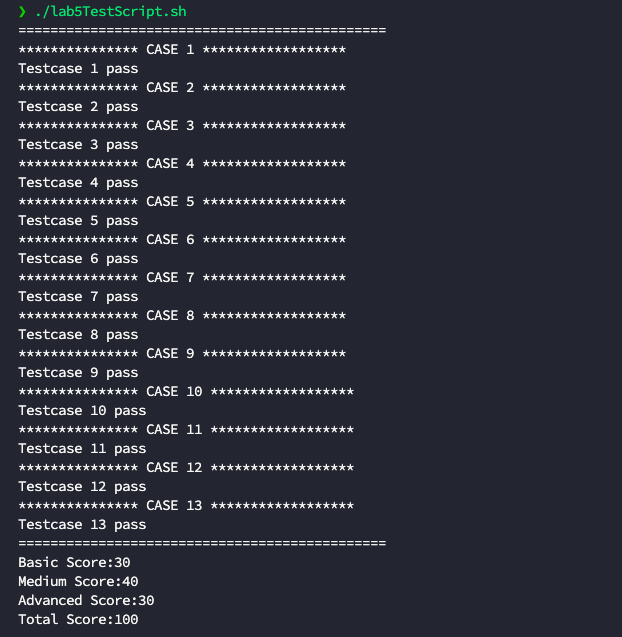
\includegraphics[width=0.5\textwidth]{result.png}
    \caption{result}
\end{figure}

\section{Difficulties and Solutions}
\begin{itemize}
    \item The pipeline registers delayed two cycles instead of 1 cycle. \\
    \textbf{\textit{Solution:}} With misunderstanding, we used internal stored registers, 
        so it took 2 cycles for an input to propagate to the output.
        We found the mistake when looking at the wave diagram during the debugging of other components,
        and in order to fix this, we find some online resources and learn how to define pipeline registers.
    \item Immediate in \verb|load| / \verb|jump| instructions is incorrect when we directly copy the code of Lab04. \\
    \textbf{\textit{Solution:}} As we mentioned in 1.4, this is cause by the presence of the shift left one unit, 
        we simply remove the padding zero in LSB to get the correct result.
    \item Cannot distinguish normal I-type instructions and Load/Store in \verb|ALU_Ctrl| \\
    \textbf{\textit{Solution:}} As the description of decoder, we forced the \verb|ALUOp| of I-type instructions to be \verb|2'b11|. 
\end{itemize}

\end{document}